\documentclass[a4paper,12pt]{article}
\usepackage{tikz}
\usetikzlibrary{arrows,shapes}

\usepackage[english]{babel}
\usepackage{courier}


\usepackage[T1]{fontenc}

\usepackage[pdftex, colorlinks=true]{hyperref}

\usepackage{listings}
\lstloadlanguages{python}
\lstset{language=python,numbers=left,numberstyle=\tiny,emph={self},emphstyle=\color{blue},basicstyle=\footnotesize}
\title{How To Become a Production Manager}
\author{S.~Poss}

\begin{document}
\tikzstyle{decision} = [diamond, draw, text badly centered, node distance=2.8cm]
\tikzstyle{block} = [rectangle, draw, text centered, rounded corners, node distance=2.2cm]
\tikzstyle{autoblock} = [rectangle, draw, text centered, rounded corners, node distance=2.2cm]
\tikzstyle{line} = [draw, -triangle 90]
\tikzstyle{dline} = [draw, dashed, -triangle 90]

\maketitle
\abstract{This document presents the method for group production managers to
extend existing productions.}

\tableofcontents

\section{Introduction}
There are at least seven different analysis being performed in parallel. There
are as many people looking at the corresponding samples. It would be more
convenient if every analysis gets a reponsible for the production. Its task is
only to extend the existing productions, not to submit new ones. 

Submission will
still be done by a very restricted set of people to ensure harmony of
production definitions. 

The defined production managers should have the right to extend, stop and
restart existing productions. This can fortunately be done  via the web
interface. The interactions with the productuion system will be detailed in the
following section, and the limitations that should be respected and eventually
enforced will be detailed in the last section.

\section{Interacting with the production system}
To interact with the system, you should first be connected with your browser
to\\
https://volcd01.cern.ch/DIRAC/ILC-Production/ilc\_user/jobs/ProductionMonitor/display

You should have something like the Fig.~\ref{fig:welcome} as a screen. If not refer to
section~\ref{sec:problem}.
\begin{figure}[h]
\begin{center}
\begin{tikzpicture}[scale=0.8,auto]
\node{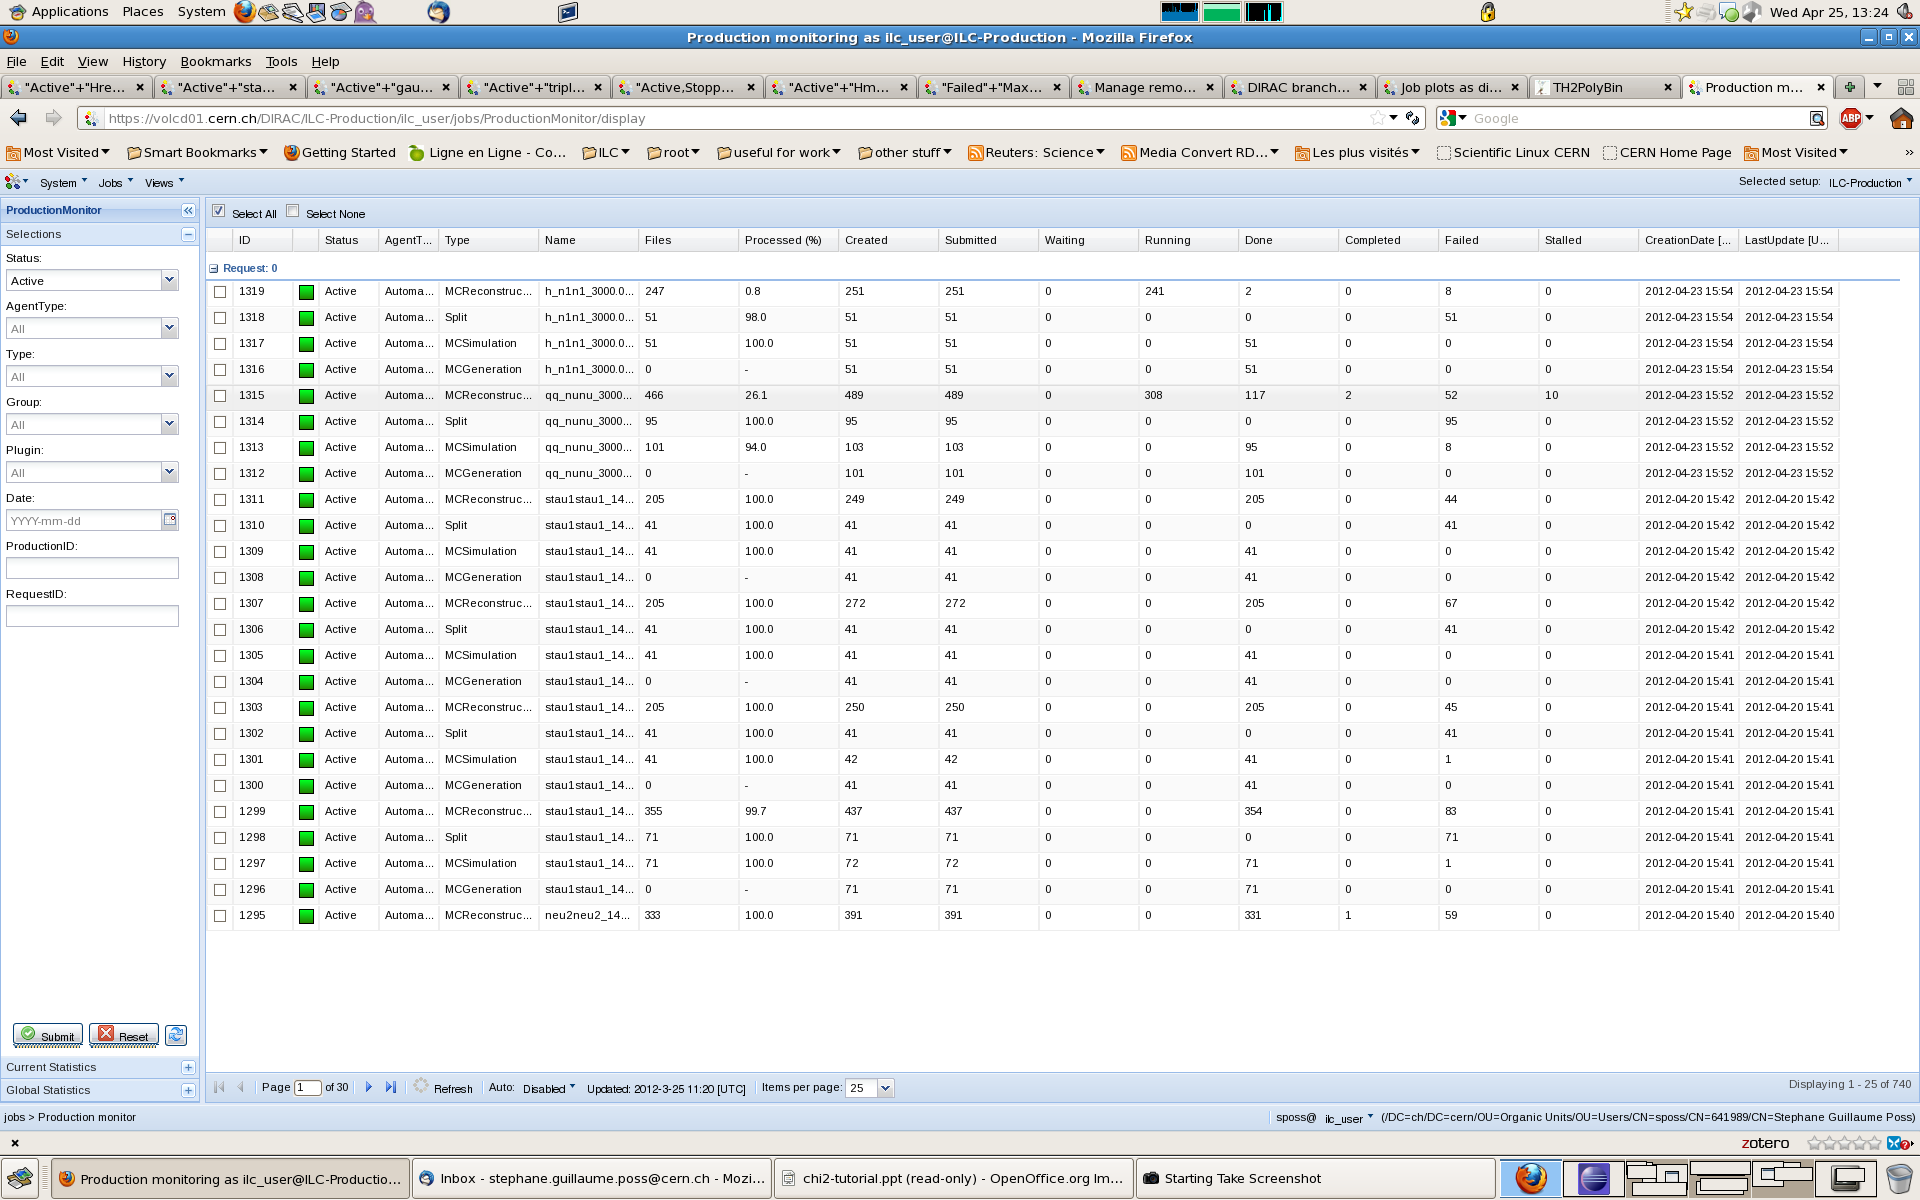
\includegraphics[width=10cm]{welcomescreen.png}};
\node{}
\end{tikzpicture}
\end{center}
\caption{Welcome screen of the production manager page.}\label{fig:welcome}
\end{figure}

What you need to do is to change the group in which you are, as most
interactions are restricted. For this you need to look at the little button
indicated in Fig.. 
\begin{figure}[h]
\begin{center}
\begin{tikzpicture}
\node {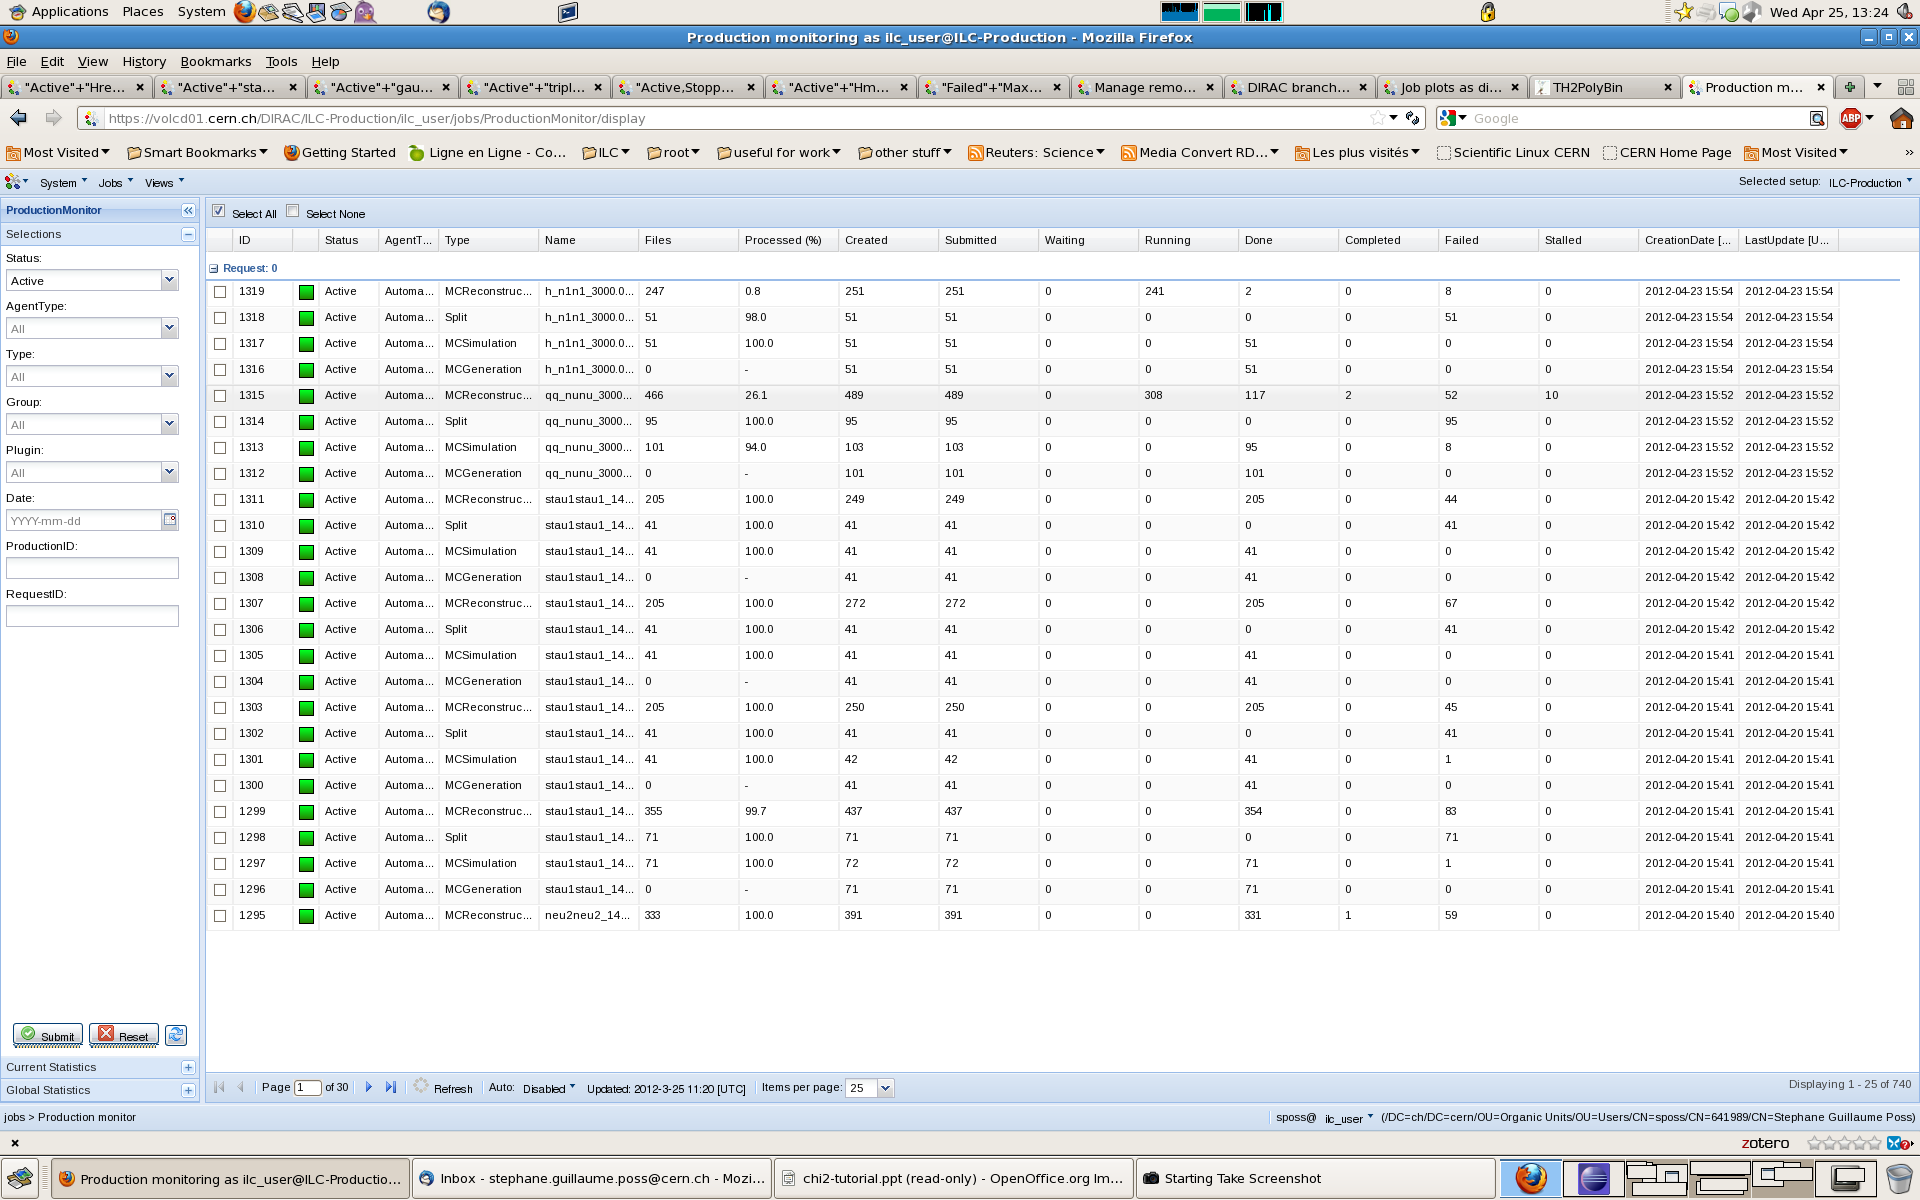
\includegraphics[width=10cm]{welcomescreen.png}};
\draw [->] (0,0) -- (1,1);
\end{tikzpicture}
\end{center}
\caption{Welcome screen of the production manager page.}\label{fig:welcome}
\end{figure}


\section{What if it does not work?}\label{sec:problem}
Well, too bad.
\end{document}